\documentclass{article}

% --- PACKAGES ---
\usepackage[utf8]{inputenc} % Handle UTF-8 input encoding
\usepackage{graphicx}       % For including images
\usepackage{amsmath}        % For advanced math typesetting
\usepackage{geometry}       % For customizing page layout
\geometry{a4paper, margin=1in}
\usepackage{hyperref}       % For creating hyperlinks in the document
\hypersetup{
	colorlinks=true,
	linkcolor=red,
	filecolor=magenta,      
	urlcolor=cyan,
}


% --- DOCUMENT INFORMATION ---
\title{Rapport - Arkanoid}
\author{David de Meester de Ravestein}
\date{\today}

% --- BEGIN DOCUMENT ---
\begin{document}

\maketitle

\begin{abstract}
Rapport dans le cadre du projet du cours INFO-F202. Reprend les informations essentielles liées au développement du jeu Arkanoid.
\end{abstract}

\tableofcontents
\newpage

\section{Tâches réalisées}

\begin{itemize}
	\item Toutes les tâches de bases ont été accomplies.
	\item Toutes les tâches additionnelles ont été accomplies.
\end{itemize}

\section{Relations classes}

\subsection{Modèle}


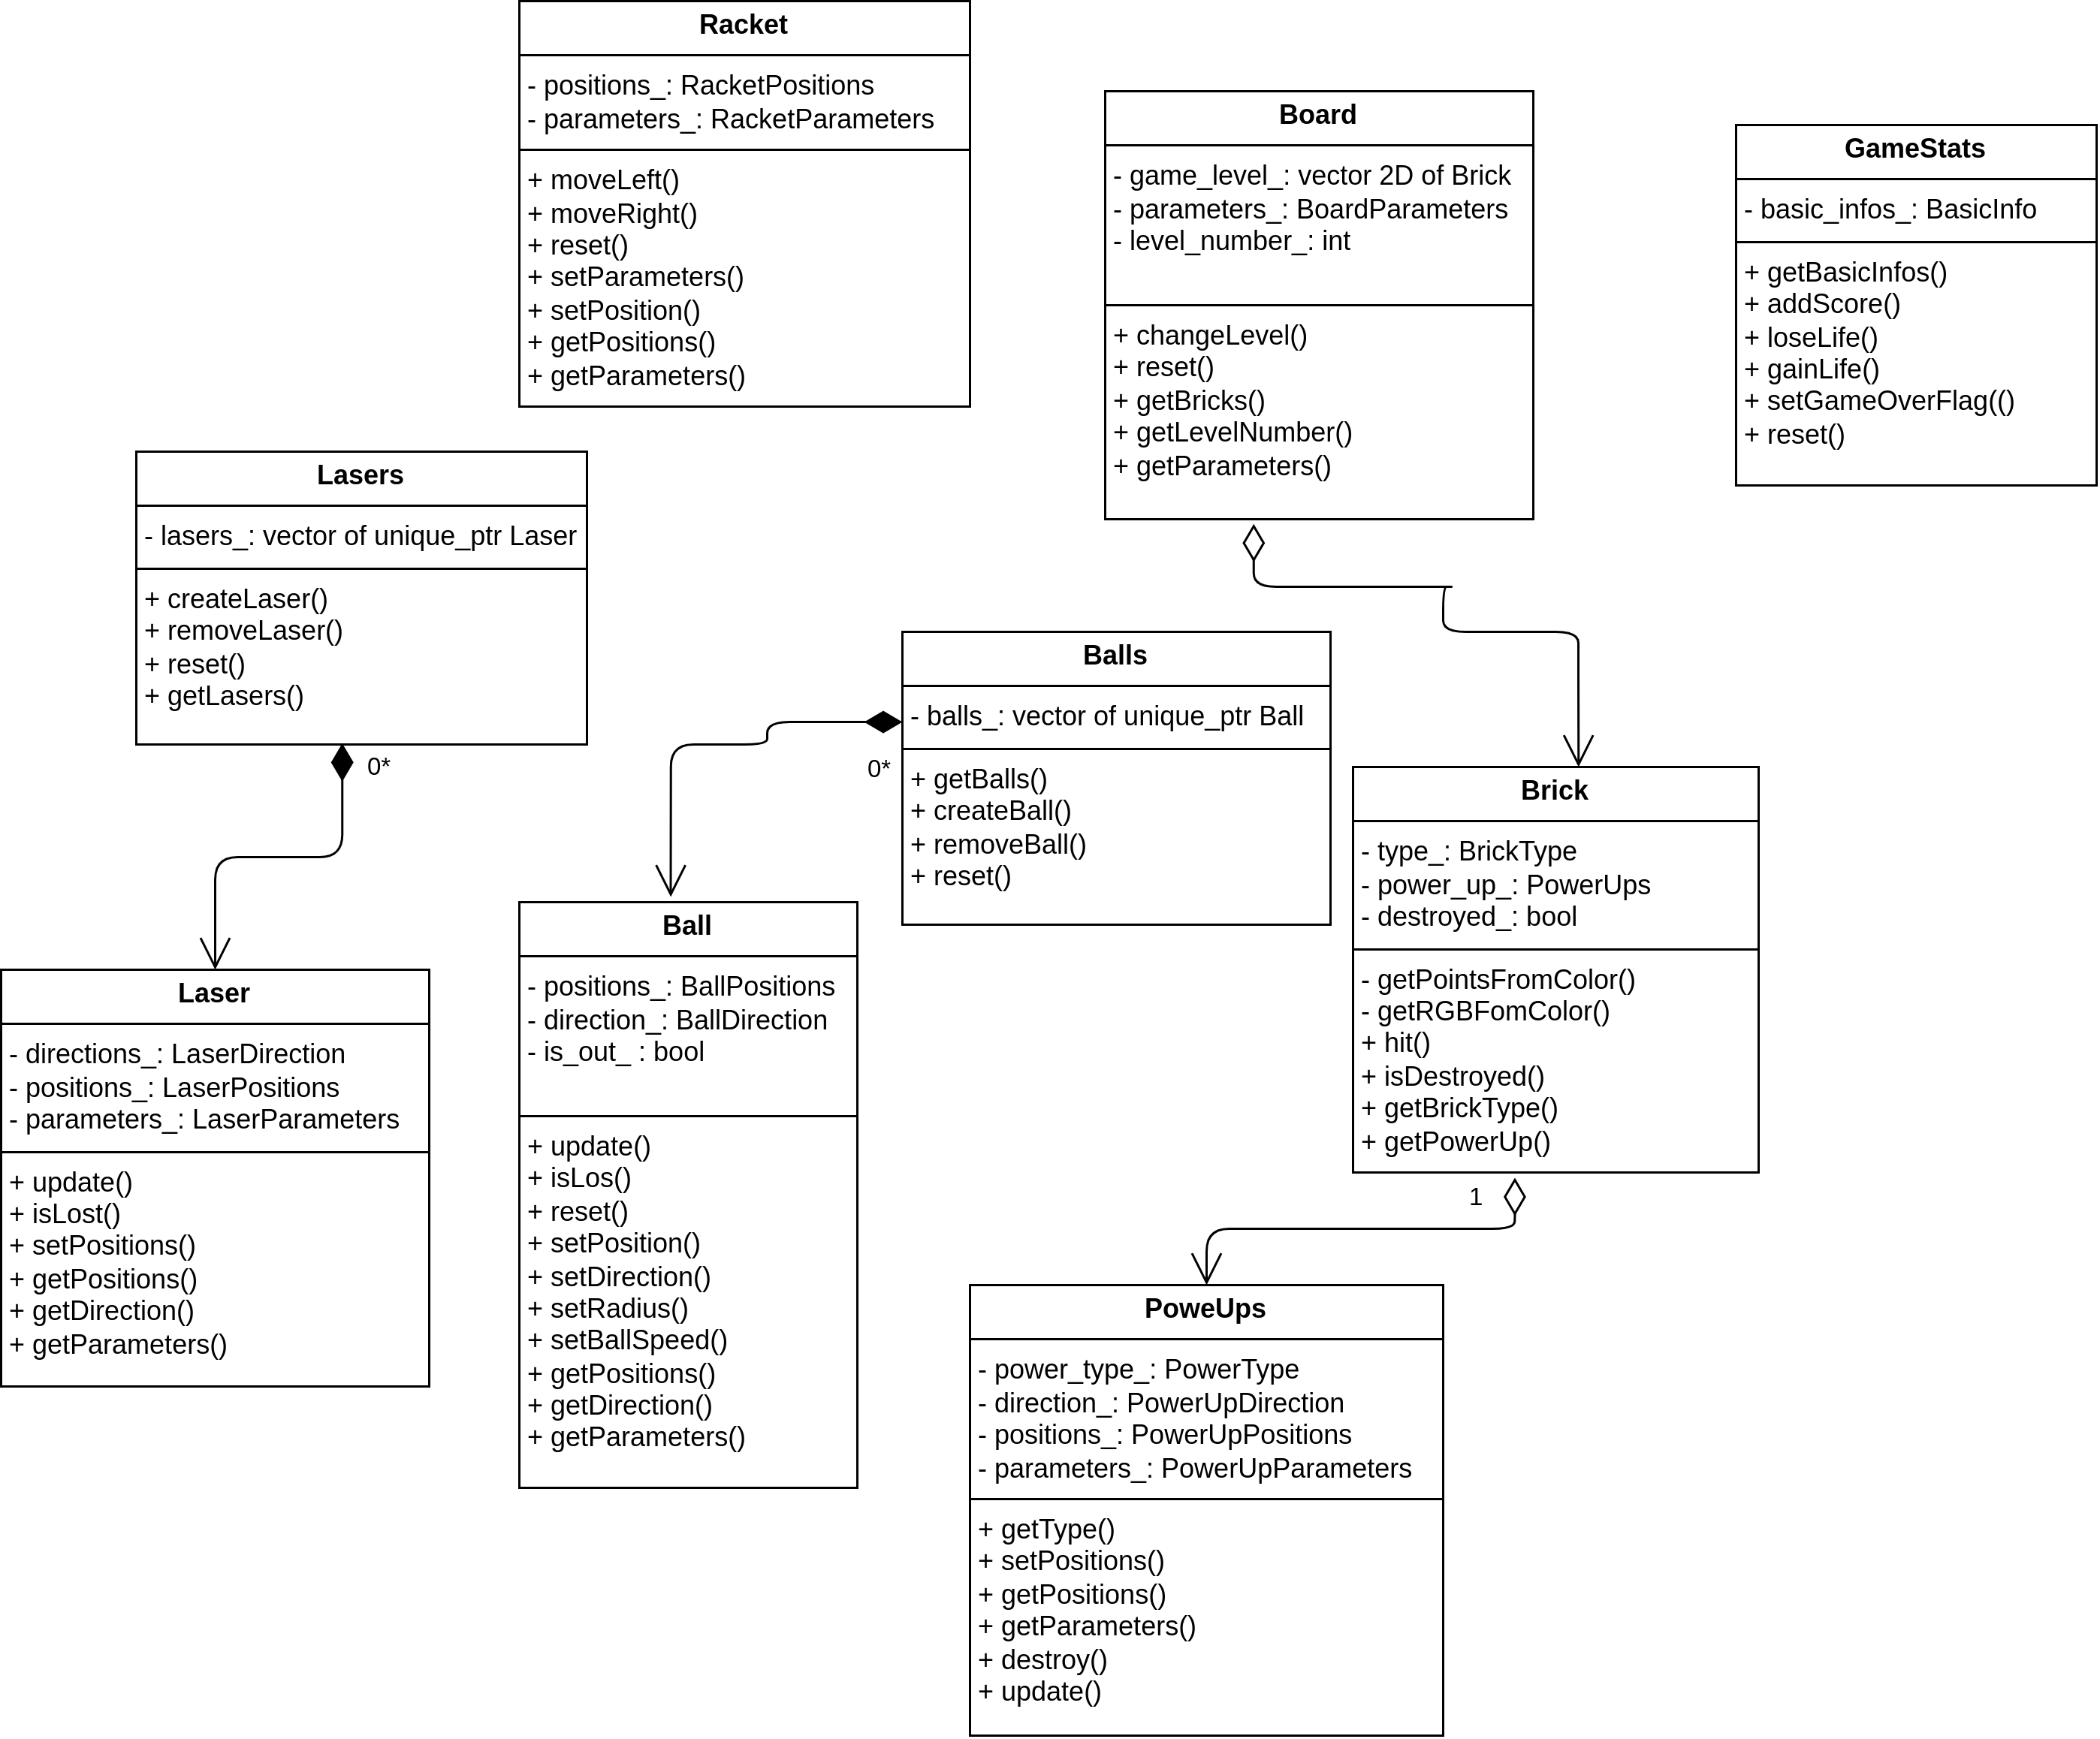
\includegraphics[width=\textwidth]{model.png}


\subsection{Vue}

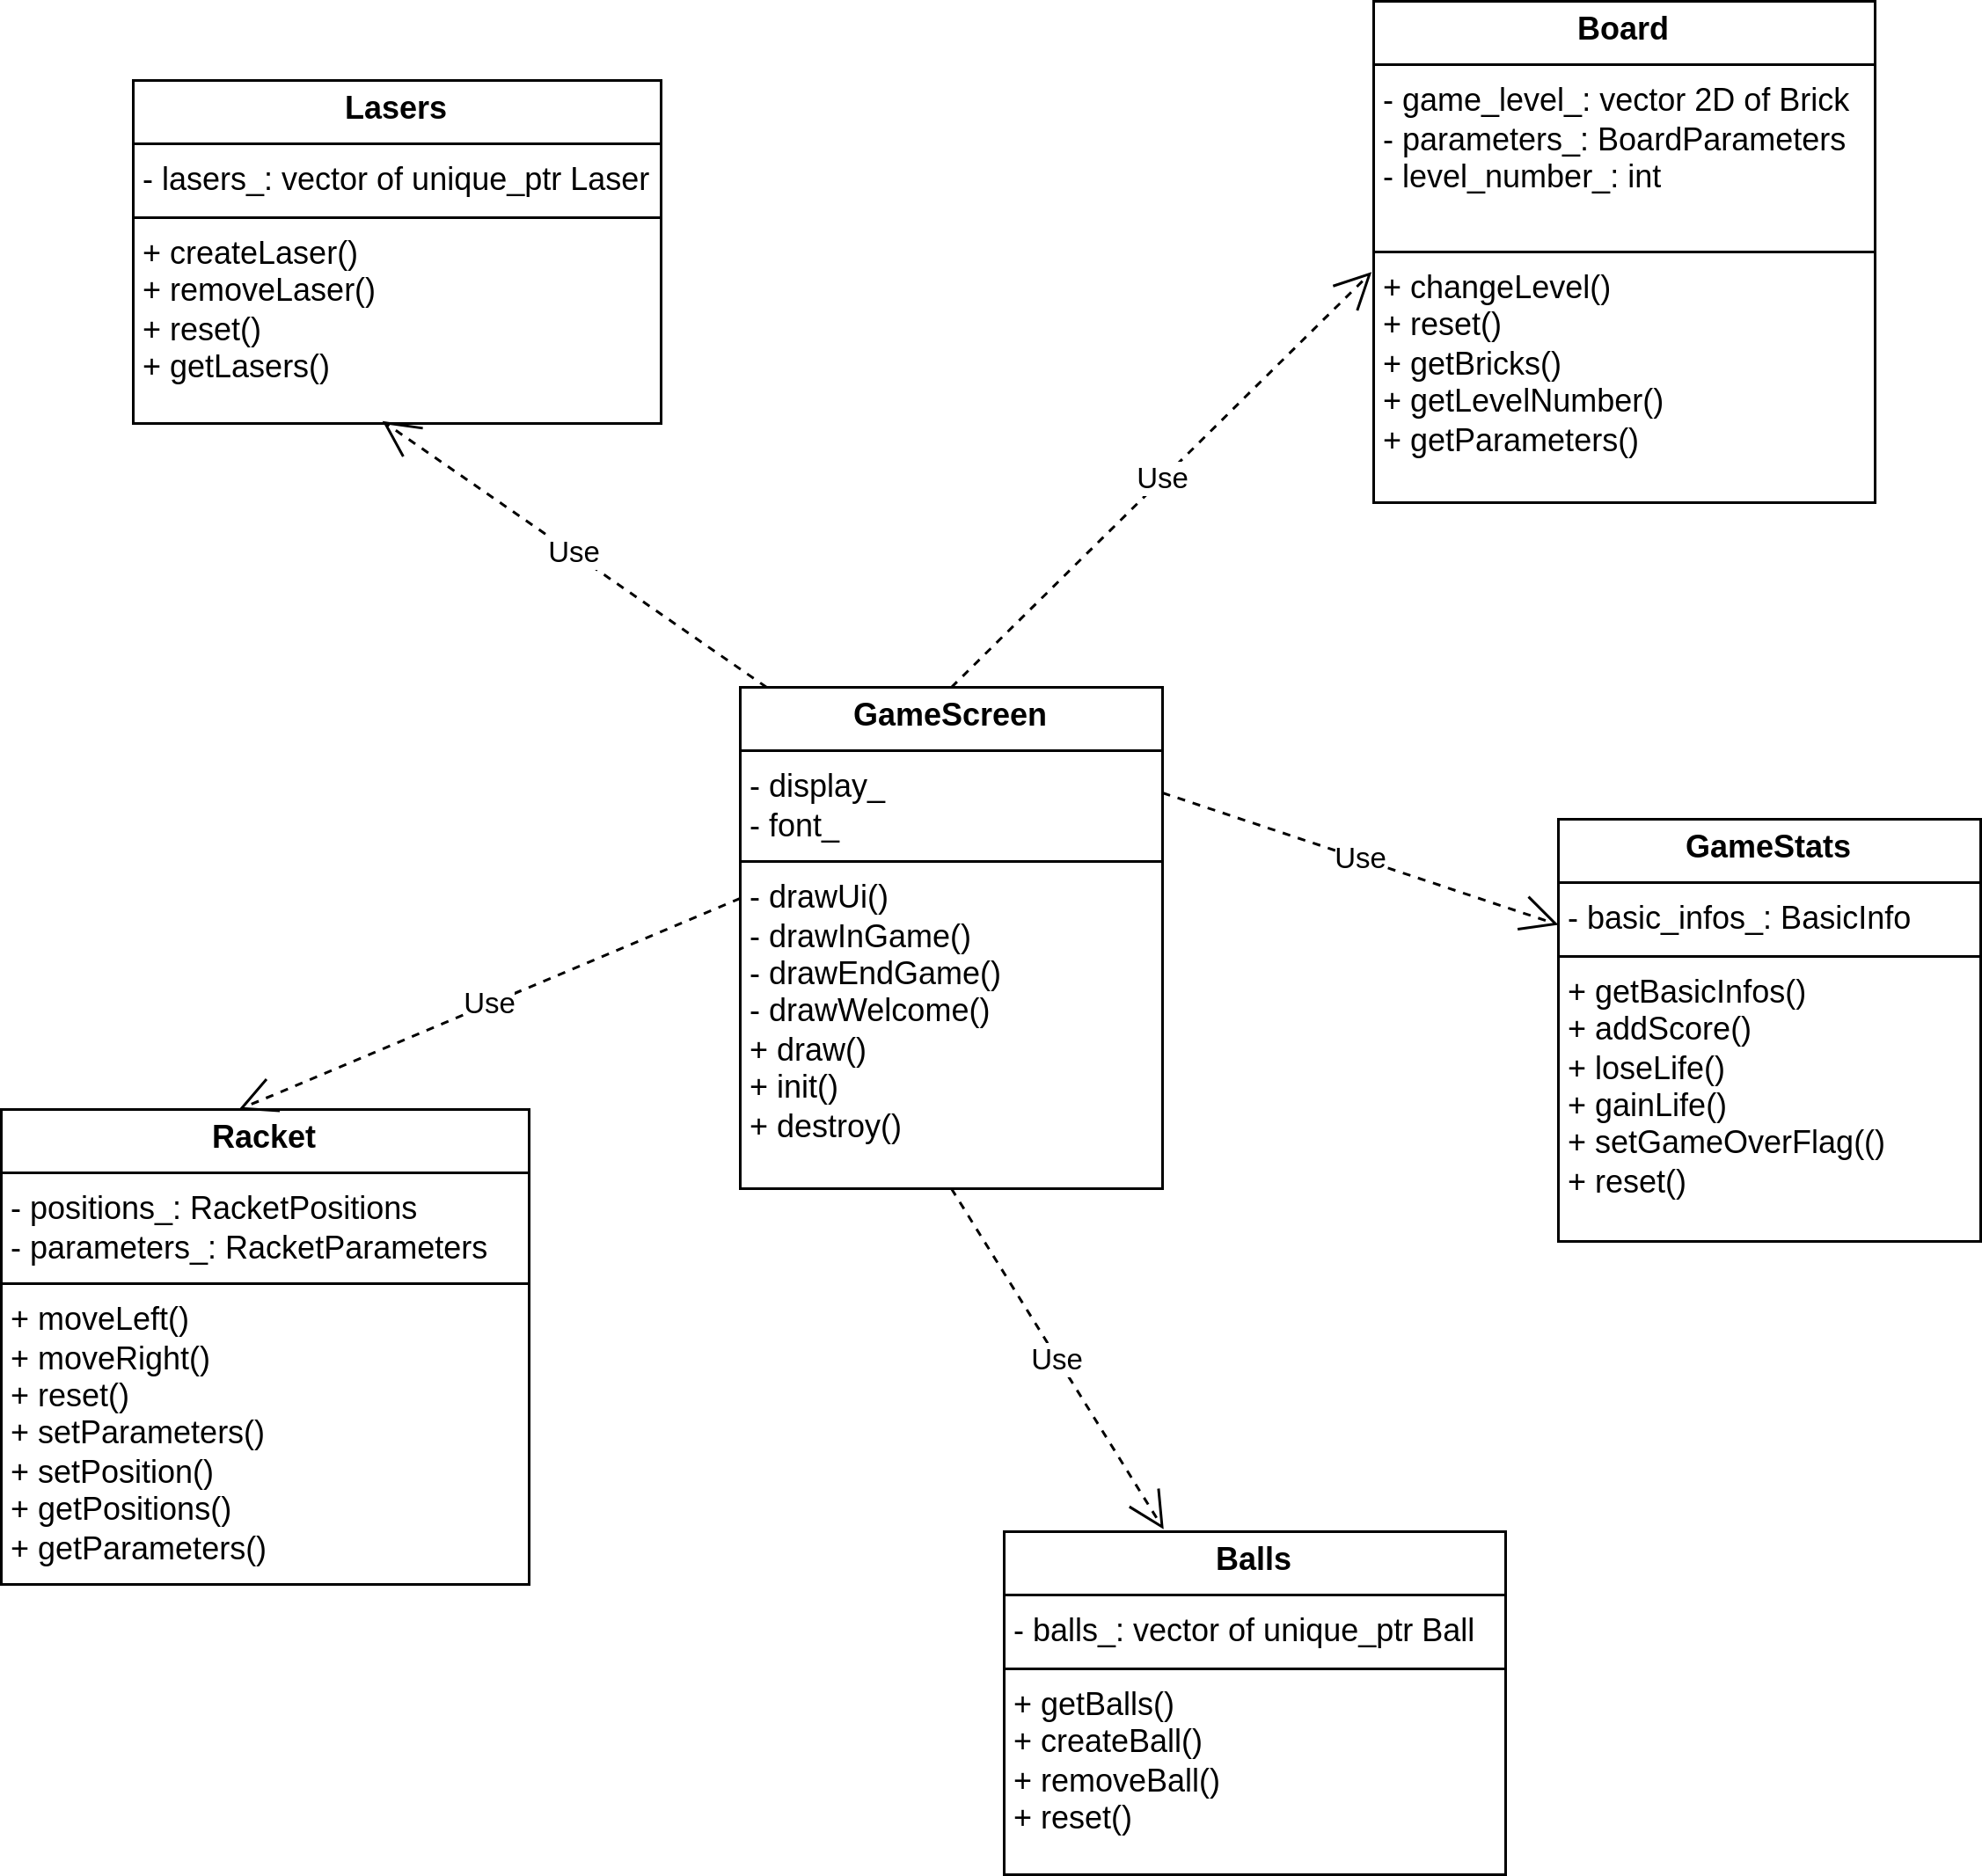
\includegraphics[width=\textwidth]{view.png}


\subsection{Controller}

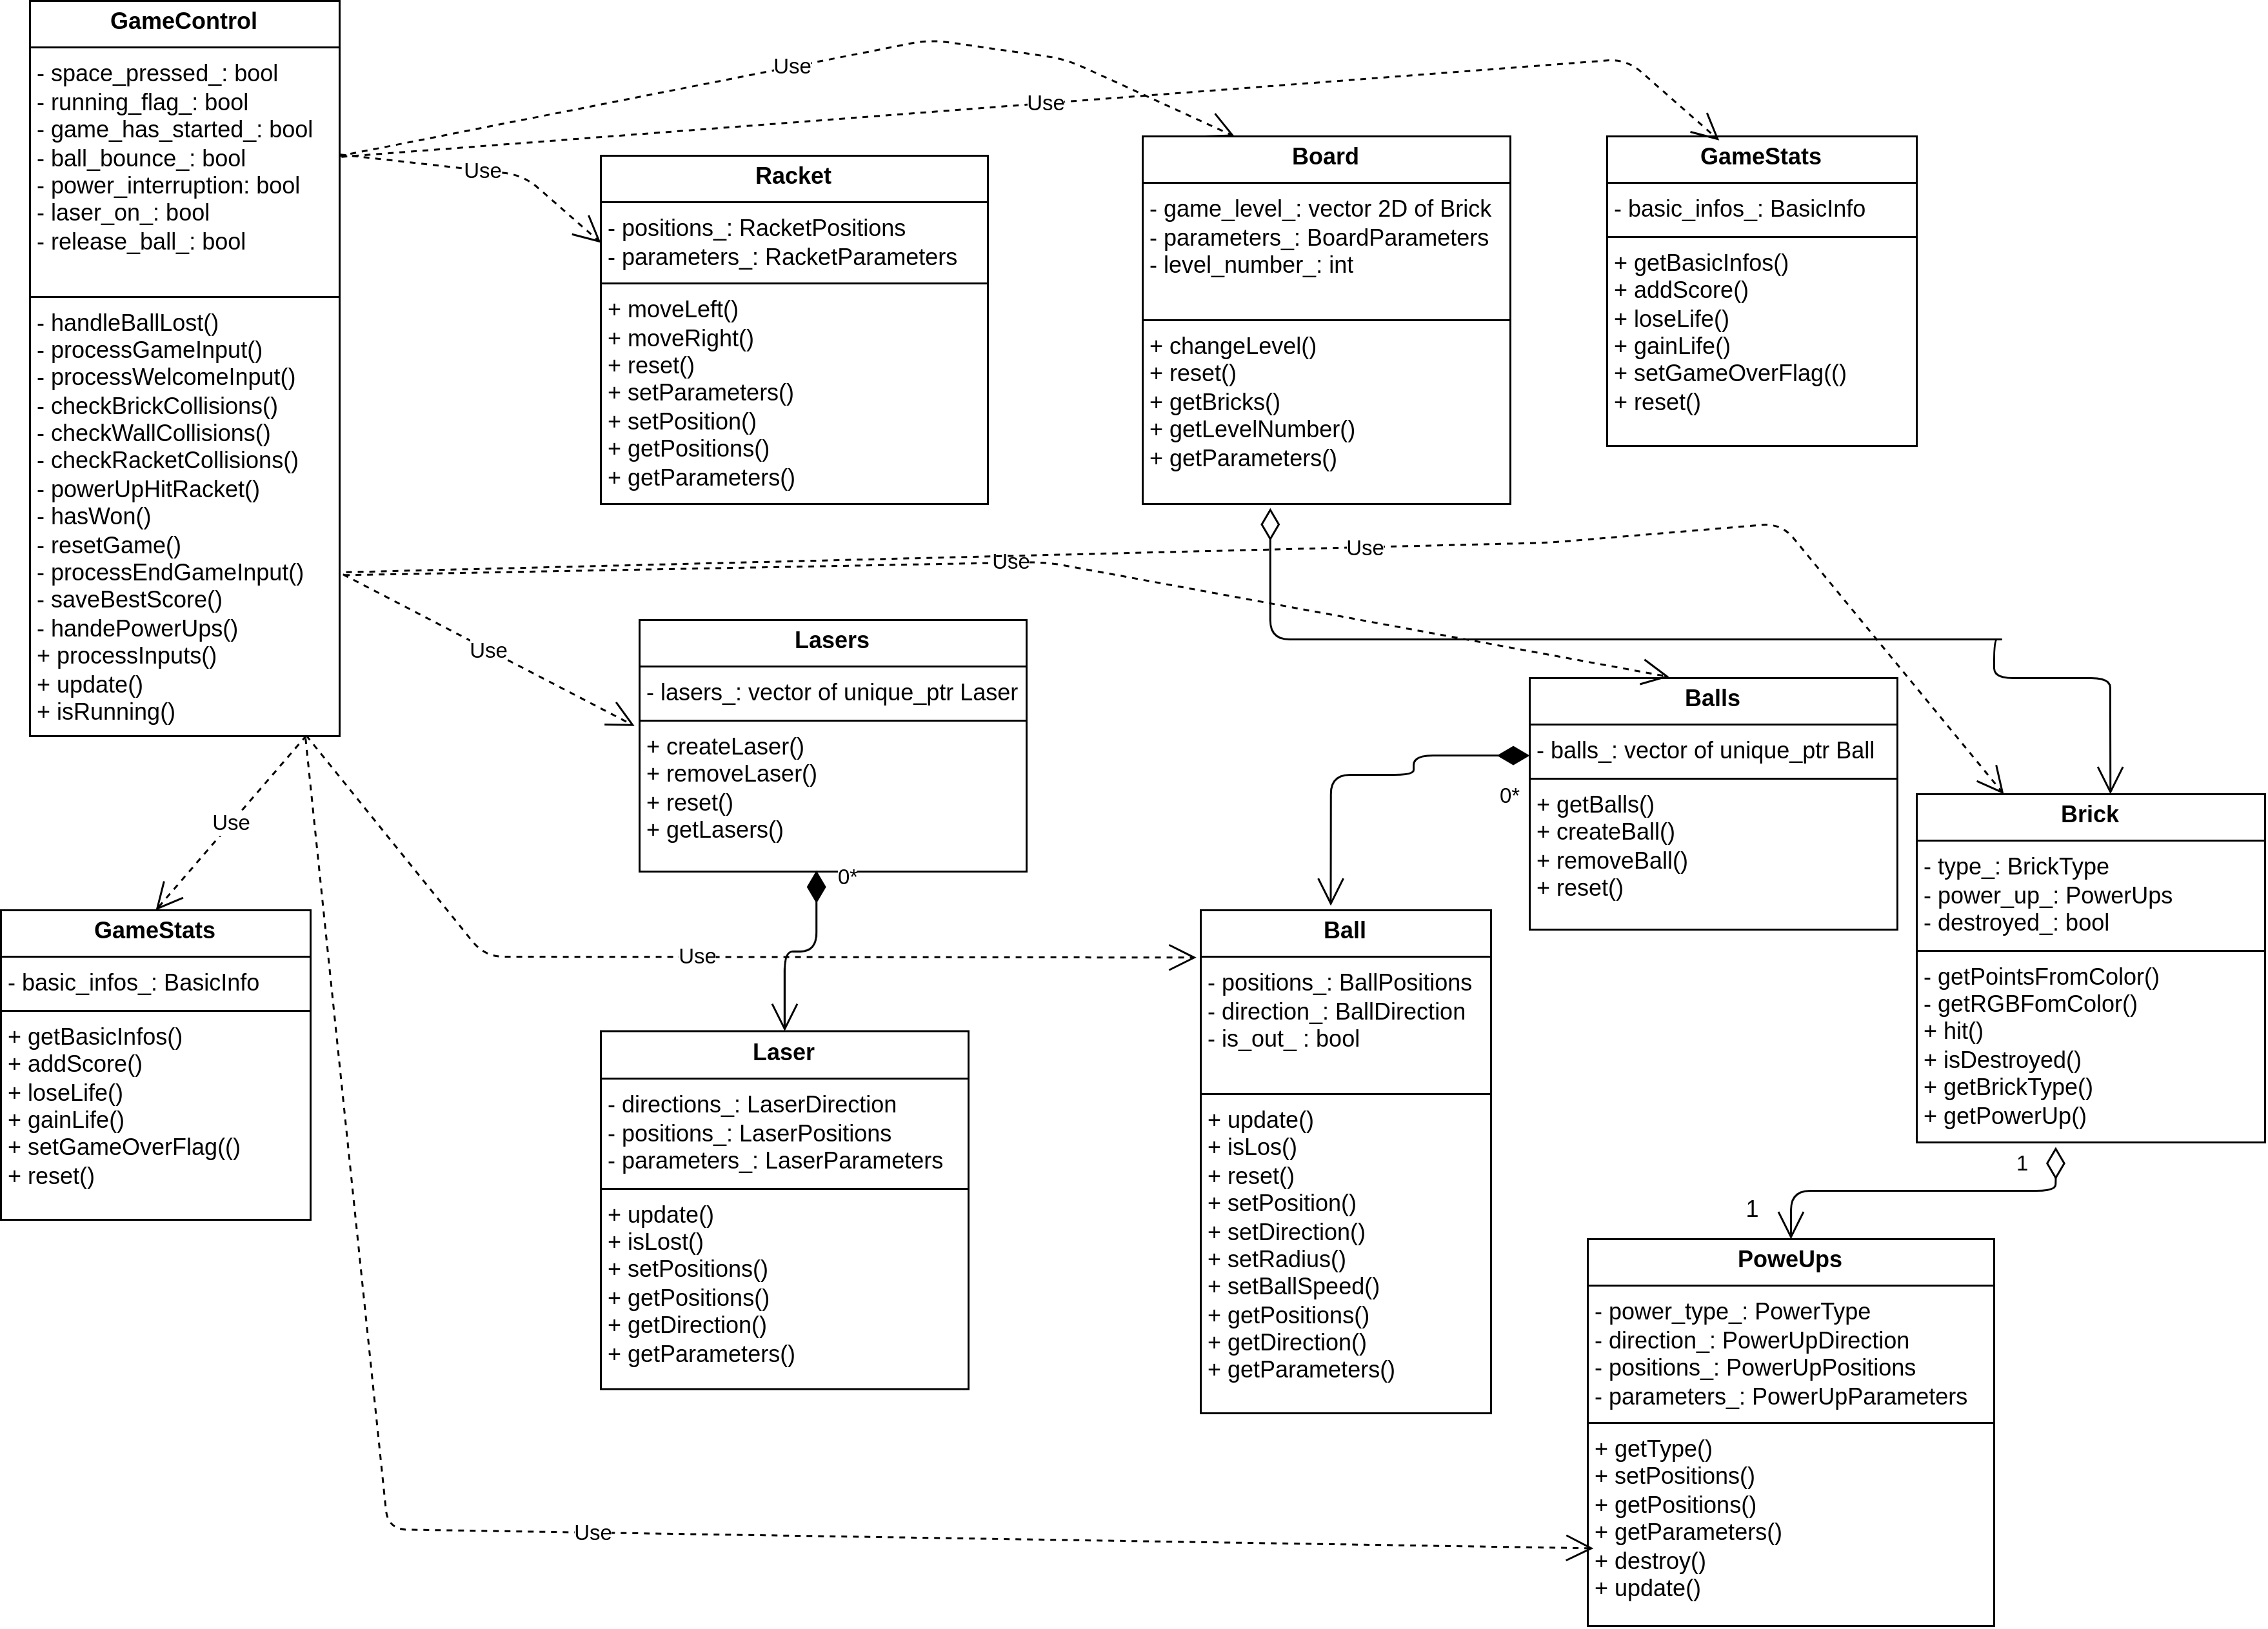
\includegraphics[width=\textwidth]{controller.png}





\section{Logique de jeu}

Le jeu commence par initialiser les composants Allegro, indispensables au bon fonctionnement du jeu. Ensuite vient la boucle principale, les inputs utilisateurs sont gérés grâce à Allegro 
et le modèle se modifie en conséquence, la raquette change de position et on met à jour le mouvement de la balle en fonction de sa direction et de sa vitesse. Tant que la variable release\_ball\_ 
est à false, la position de la balle est accrochée à la raquette. Une fois que le controller a pris les inputs et a changé le modèle, il est temps d'afficher. La vue s'en occupe grâce au fonctions
draw dédiées aux différents états de jeu. Dans le controller, à chaque update on vérifie le vecteur 2D qui représente les briques, et on regarde si il y a eu collision avec la balle. On fait de même 
pour les collisions avec le mur, le plafond et la raquette puis on affiche. Ainsi la boucle et bouclée et rebelote jusqu'à ce que l'on change d'état de jeu et quitte le jeu, la boucle principale.

\section{MVC}

La structure de code respecte le principe Modèle, Vue, Controller. Les fichiers sont triés dans les dossiers correspondants et l'utilisation des fichers respecte la catégorie dans laquelle il s'y figure.

\subsection{Modèle}

Le Modèle s'occupe de tous les objects manipulés et affichés du jeu.

\subsection{Vue}

La Vue s'occupe de prendre les objets du modèle et de les afficher grâce à la librairie Allegro.

\subsection{Controller}

Le Controller s'occupe de prendre les inputs utilisateur et de modifier le modèle en conséquence ainsi que de mettre à jour les objets au cours du temps.

\section{Copilot}

Github Copilot a été utilisé lors du développement du jeu. Je me suis retrouvé seul à devoir construire le jeu et copilot m'a aidé à être plus aguéri lors de prise de décisions. 
Il m'a également été utile pour la documentation et le refactoring qui permet une maintenance et une lisibilité de bien meilleure qualité.

% --- END DOCUMENT ---
\end{document}































